\chapter{$h^-\to \tau^-\nu_{\tau}$}
Author: Andr\'es Felipe Estrada Guerra


Description of the processes to be calculated: $h^-\to \tau^-\nu_{\tau}$

\section{Preliminares}

El Lagrangiano utilizado en (1) está dado por
\begin{eqnarray}\label{lagrangiano-1}
-\mc{L}_Y=\Bar{L}_i(\Pi_a)_{ij}H_ae_{R_j}+\epsilon_{\alpha\beta}\Bar{L}^\alpha_if_{ij}C(\Bar{L})^\beta_jh^-+\mbox{H.c},
\end{eqnarray}
en donde $L_i$ son dobletes leptónicos, $e_{R_j}$ son singletes leptónicos, $C$ es el operador de conjugación de carga, $\Pi_a$
($a=1,2$) y $f$ son matrices $3\times3$ en el espacio de sabor, $\epsilon_{\alpha\beta}$ ($\alpha,\beta=1,2$) es el tensor
antisimétrico para SU(2)$_L$ y $i,j=1,2,3$ son los índices de familia. La matriz $f$ es antisimétrica debida a la estadística de
Fermi.\\
En los eigenestados de masa para los escalares cargados, el lagrangiano anterior se escribe de la siguiente manera:
\begin{eqnarray}\label{lagrangiano-2}
-\mc{L}_Y  & \supset & \Bar{\nu}_{L_i'}O_{i'j}e_{R_j}(h_1^+\cos\varphi -h_2^+\sin\varphi) \nonumber \\
& & +(\nu_{L_i})^TC(2f_{ij})e_{L_j}(h_1^+\sin\varphi +h_2^+\cos\varphi)+\mbox{H.c.},
\end{eqnarray}
en donde $W_{11}=W_{22}=\cos\varphi$ y $W_{12}=-W_{21}=\sin\varphi$.\\
Estoy interesado en  el decaimiento del escalar cargado $h_1^+$ en dos leptones: $\nu_\tau$ y $\Bar{\tau}$. Por lo tanto, la
parte del lagrangiano anterior que describe este decaimiento está dado por:
\begin{eqnarray}\label{lagrangiano-3}
\mc{L}_Y&=&-(\nu_{L_i})^TC(2f_{ij})e_{L_j}h_1^+\sin\varphi +\mbox{H.c.} \nonumber \\
&=&-(\nu_{L_i})^T(2f_{ij})\Bar{e}_{L_j}h_1^+\sin\varphi +\mbox{H.c.},
\end{eqnarray}
por lo que el Hamiltoniano es:
\begin{eqnarray}\label{hamilton-1}
H=(\nu_{L_i})^T(2f_{ij})\Bar{e}_{L_j}h_1^+\sin\varphi +\mbox{H.c.}.
\end{eqnarray}
%En la siguiente figura se ilustra el proceso bajo estudio:
%\begin{center}
%\begin{figure}[h]
 %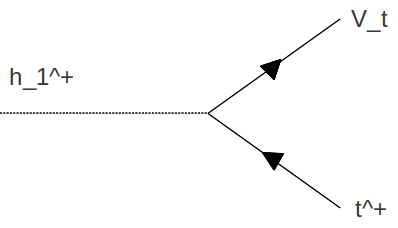
\includegraphics[scale=1]{grafica.png}
 %\caption{Grafica del proceso $h_1^+(k)\,\rightarrow\,v_\tau(k)\,\tau^+(p)$.}
%\end{figure}
%\end{center}
La matriz $S$ a primer orden está dada por:
\begin{eqnarray}\label{s-matriz-1}
S^{(1)}&=&\mc{T}\left[-i\int d^4x\,:\mc{H}:\right] \nonumber \\
&=&-i(2f)\sin\varphi\int d^4x\,:\psi(x)\Bar{\psi}(x)\phi(x): ,
\end{eqnarray}
en donde se ha omitido el símbolo de ordenamiento temporal, debido a que existe un solo punto en el espacio-tiempo y, por lo
tanto, un solo tiempo. Debido a esto, el teorema de Wick no es necesario para este orden de la matriz $S$.\\
Ahora bien, la descomposición de Fourier para los campos involucrados está dada por:
\begin{eqnarray}\label{fourier-campos-1}
\phi(x)&=&\int\frac{d^3p}{\sqrt{(2\pi)^32E_p}}\left[a(\vtr{p})e^{-ip\cdot x}+a^\dagger(\vtr{p})e^{ip\cdot x}\right] \nonumber \\
&=&\phi_++\phi_-, \nonumber \\
\psi(x)&=&\int\frac{d^3p}{\sqrt{(2\pi)^32E_p}}\sum_{s=1,2}\left[f_s(\vtr{p})u_s(\vtr{p})e^{-ip\cdot
x}+\hat{f}_s^\dagger(\vtr{p})v_s(\vtr{p})e^{ip\cdot x}\right] \nonumber \\
&=&\psi_++\psi_-, \nonumber \\
\bar{\psi}(x)&=&\int\frac{d^3p}{\sqrt{(2\pi)^32E_p}}\sum_{s=1,2}\left[f_s^\dagger(\vtr{p})\bar{u}_s(\vtr{p})e^{ip\cdot
x}+\hat{f}_s(\vtr{p})\bar{v}_s(\vtr{p})e^{-ip\cdot x}\right] \nonumber \\
&=&\bar{\psi}_-+\bar{\psi}_+.
\end{eqnarray}
Los estados de una sola partícula están definidos de la siguiente manera:
\begin{equation}
  \label{estados-1-part-1}
\begin{split}
\ketm{h_1^+(\vtr{k})}&=\sqrt{\frac{(2\pi)^3}{V}}a^\dagger(\vtr{k})\ketm{0} \\
\ketm{\nu_\tau(\vtr{k},s)}&=\sqrt{\frac{(2\pi)^3}{V}}f_s^\dagger(\vtr{k})\ketm{0} \\
\ketm{\tau^+(\vtr{p},s)}&=\sqrt{\frac{(2\pi)^3}{V}}\Hat{f}_s^\dagger(\vtr{p})\ketm{0}. 
\end{split}
\end{equation}
Utilizando las relaciones de conmutación y anticonmutación entre los operadores de creación y destrucción:
\begin{eqnarray*}
\conmu{a(\vtr{k})}{a(\vtr{k}')}&=&\delta^3(\vtr{k}-\vtr{k}') \\
\aconmu{f_s(\vtr{k})}{f_{s'}^\dagger(\vtr{k}')}&=&\delta_{ss'}\delta^3(\vtr{k}-\vtr{k}') \\
\aconmu{\hat{f}_s(\vtr{p})}{\hat{f}_{s'}^\dagger(\vtr{p}')}&=&\delta_{ss'}\delta^3(\vtr{p}-\vtr{p}'),
\end{eqnarray*}
se llega entonces a que los estados de una sola partícula están normalizados de la siguiente manera:
\begin{eqnarray*}
\prodin{h_1^+(\vtr{k})}{h_1^+(\vtr{k}')}&=&\frac{(2\pi)^3}{V}\delta^3(\vtr{k}-\vtr{k}')\\
\prodin{\nu_\tau(\vtr{k},s)}{\nu_\tau(\vtr{k}',s')}&=&\frac{(2\pi)^3}{V}\delta_{ss'}\delta^3(\vtr{k}-\vtr{k}')\\
\prodin{\tau^+(\vtr{p},s)}{\tau^+(\vtr{p}',s')}&=&\frac{(2\pi)^3}{V}\delta_{ss'}\delta^3(\vtr{p}-\vtr{p}').
\end{eqnarray*}
Tal como se demuestra en las notas del curso, es conveniente trabajar en el límite discreto, en donde:
\begin{eqnarray*}
\delta^3(0)_p=\frac{V}{(2\pi)^3}.
\end{eqnarray*}
Con esta definición, los estados de una sola partícula en (\ref{estados-1-part-1}) están normalizados a la unidad, siempre y
cuando se tome el límite de $V\rightarrow \infty$ al final del cálculo de cualquier cantidad física.\\
La acción de los operadores de campo sobre los estados de una partícula están dados por:
\begin{eqnarray}\label{accion-operadores-campos-1}
\phi_+(x)\ketm{h_1^+(\vtr{k})}&=&\int\frac{d^3p}{\sqrt{(2\pi)^32\omega_p}}a(\vtr{p})e^{-ip\cdot
x}\sqrt{\frac{(2\pi)^3}{V}}a^\dagger(\vtr{k})\ketm{0} \nonumber \\
&=&\int\frac{d^3p}{2\omega_pV}\left[a^\dagger(\vtr{k})a(\vtr{p})+\delta^3(\vtr{p}-\vtr{k})\right]e^{-ip\cdot x}\ketm{0} \nonumber \\
&=&\frac{1}{\sqrt{2\omega_kV}}e^{-ik\cdot x}\ketm{0}, \nonumber \\
\psi_+(x)\ketm{\nu_\tau(\vtr{k},s)}&=&\int\frac{d^3p}{\sqrt{(2\pi)^32\omega_p}}\sum_{s'=1,2}f_{s'}(\vtr{p})u_{s'}(\vtr{p})e^{
-ip\cdot x}\sqrt{\frac{(2\pi)^3}{V}}f_s^\dagger(\vtr{k})\ketm{0} \nonumber \\
&=&\int\frac{d^3p}{\sqrt{2\omega_pV}}\sum_{s'=1,2}\left[-f_s^\dagger(\vtr{k})f_{s'}(\vtr{p})+\delta_{ss'}\delta^3(\vtr{k}-\vtr{p}
)\right ] u_{s'}(\vtr{p})e^{-ip\cdot x}\ketm{0} \nonumber \\
&=&\frac{1}{\sqrt{2\omega_kV}}u_s(\vtr{k})e^{-ik\cdot x}\ketm{0},\nonumber \\
\Bar{\psi}_+(x)\ketm{\tau^+(\vtr{p},s)}&=&\int\frac{d^3p'}{\sqrt{(2\pi)^32E_{p'}}}\sum_{s'=1,2}\hat{f}_{s'}(\vtr{p}')\Bar{v}_{s'}
(\vtr { p}')e^{-ip'\cdot x}\sqrt{\frac{(2\pi)^3}{V}}\Hat{f}_s(\vtr{p})\ketm{0}\nonumber \\
&=&\frac{1}{\sqrt{2E_pV}}\Bar{v}_s(\vtr{p})e^{-ip\cdot x}\ketm{0}.
\end{eqnarray}
De manera totalmente análoga se obtiene para los operadores adjuntos:
\begin{eqnarray}\label{accion-operadores-campos-2}
\left<h_1^+(\vtr{k})\right|\phi_-(x)&=&\frac{1}{\sqrt{2\omega_kV}}e^{ik\cdot x}\left<0\right|, \nonumber \\
\left<\nu_\tau(\vtr{k},s)\right|\Bar{\psi}_-(x)&=&\frac{1}{\sqrt{2\omega_kV}}\Bar{u}_s(\vtr{k})e^{ik\cdot x}\left<0\right|, \nonumber \\
\left<\tau^+(\vtr{p},s)\right|\psi_-(x)&=&\frac{1}{\sqrt{2E_pV}}v_s(\vtr{p})e^{ip\cdot x}\left<0\right|.
\end{eqnarray}
El estado inicial $\ketm{i}$ y final $\ketm{f}$ del proceso están dados por:
\begin{eqnarray*}
\ketm{i}=\ketm{h_1^+(\vtr{k})}, \quad \ketm{f}=\ketm{\tau^+(\vtr{p},s),\nu_\tau(\vtr{k}',s')}.
\end{eqnarray*}
De la expresión (\ref{s-matriz-1}) se tiene lo siguiente:
\begin{eqnarray*}
:\psi\bar{\psi}\phi:&=&:(\psi_++\psi_-)(\bar{\psi}_++\bar{\psi}_-)(\phi_++\phi_-): \\
&=&:(\psi_+\bar{\psi}_+ +\psi_+\bar{\psi}_- +\psi_-\bar{\psi}_+ +\psi_-\bar{\psi}_-)(\phi_++\phi_-): \\
&=&:\psi_+\bar{\psi}_+\phi_- +\psi_+\bar{\psi}_+\phi_- +\psi_+\bar{\psi}_-\phi_+ + \psi_+\bar{\psi}_-\phi_- +
\psi_-\bar{\psi}_+\phi_+ \\
& & +\psi_-\bar{\psi}_+\phi_- +\psi_-\bar{\psi}_-\phi_+ +\psi_-\bar{\psi}_-\phi_-:
\end{eqnarray*}
y por lo tanto, el único término que contribuye al elemento matricial del proceso es cuestión es:
\begin{eqnarray*}
-i(2f)\sin\varphi\int d^4x\,\psi_-\bar{\psi}_-\phi_+
\end{eqnarray*}

\section{Cálculo del elemento matricial}

Teniendo en cuenta la expresión anterior, se tiene entonces que:
\begin{eqnarray}\label{calculo-1}
S_{fi}^{(1)}&=&-i(2f)\sin\varphi\int
d^4x\,\braket{\tau^+(\vtr{p},s),\nu_\tau(\vtr{k}',s')}{\psi_-\bar{\psi}_-\phi_+}{h_1^+(\vtr{k})},
\end{eqnarray}
y haciendo uso de las expresiones (\ref{accion-operadores-campos-1}) y (\ref{accion-operadores-campos-2}), obtenemos:
\begin{eqnarray}\label{calculo-2}
S_{fi}^{(1)}&=&-i(2f)\sin\varphi v_{s}(\vtr{p})\bar{u}_{s'}(\vtr{k}')\nonumber \\
& &\times \int d^4x\,e^{i(p+k'-k)\cdot
x}\frac{1}{\sqrt{2E_pV}}\frac{1}{\sqrt{2\omega_{k'}V}}\frac{1}{\sqrt{2\omega_kV}}.
\end{eqnarray}
En la integración sobre $x$, se tiene en cuenta la condición $V\rightarrow\infty$, y por lo tanto:
\begin{eqnarray*}
\int d^4x\,e^{i(p+k'-k)\cdot x}=(2\pi)^4\delta^4(k-k'-p),
\end{eqnarray*}
y colocando esto en la expresión (\ref{calculo-2}):
\begin{eqnarray}\label{calculo-3}
S_{fi}^{(1)}&=&\left[-i(2f)\sin\varphi\right]\left[v_s(\vtr{p})\bar{u}_{s'}(\vtr{k}')\right]\left[(2\pi)^4\delta^4(k-k'-p)\right]
 \nonumber \\
& &\times\left [ \frac { 1 } { \sqrt { 2E_pV } } \frac { 1 }{\sqrt{2\omega_{k'}V}}\frac{1}{\sqrt{2\omega_kV}}\right]
\end{eqnarray}


\section{Tasa de decaimiento}
Para una partícula que decae en cierto número de partículas en el estado final, suponiendo que los estados inicial y final son
diferentes, el elemento matricial $S$ se puede escribir como
\begin{eqnarray}\label{elem-matricial-s-gen}
S_{fi}=i(2\pi)^4\delta^4(p_i-\sum_{f}p_f)\frac{1}{\sqrt{2E_iV}}\prod_f\frac{1}{\sqrt{2E_fV}}\mc{M}_{fi},
\end{eqnarray}
siendo $i\mc{M}_{fi}$ la amplitud de Feynmann. Comparando la expresión anterior con la dada en (\ref{calculo-3}), tenemos que:
\begin{eqnarray}\label{amplitud-feynmann-1}
i\mc{M}_{fi}^{(1)}=-i(2f)\sin\varphi\,v_s(\vtr{p})\bar{u}_{s'}(\vtr{k}').
\end{eqnarray}
La probabilidad de transición del estado inicial al estado final está dada por $\left|S_{fi}^{(1)}\right|^2$, luego:
\begin{eqnarray}\label{prob-transicion-1}
\left|S_{fi}^{(1)}\right|^2=(2\pi)^4\delta^4\left(k-k'-p\right)VT\frac{1}{2\omega_kV}\frac{1}{2\omega_{k'}V}\frac{1}{2E_pV}
\left|\mc{M}_{fi}^{(1)}\right|^2.
\end{eqnarray}
La probabilidad de transición por unidad de tiempo se obtiene dividiendo la expresión anterior por $T$, que da como resultado:
\begin{eqnarray}\label{prob-transicion-tiempo-1}
\frac{\left|S_{fi}^{(1)}\right|^2}{T}=(2\pi)^4\delta^4\left(k-k'-p\right)\frac{1}{2\omega_k}\frac{1}{2\omega_{k'}V}\frac{1}{
2E_pV}
\left|\mc{M}_{fi}^{(1)}\right|^2.
\end{eqnarray}
Esta es la probabilidad por unidad de tiempo de obtener un estado final con valores específicos del momento. Cuando se utiliza el
límite $V\rightarrow\infty$, los valores del momento caen en el continuo, por lo que no se buscan valores específicos del
momento, sino más bien por momentos finales en algún rango específico. Esto se realiza discretizando el espacio de fases en
celdas de volumen $(2\pi\hbar)^3=(2\pi)^3$ ($\hbar=1$ en unidades naturales) y colocando un estado en cada celda. Por lo tanto,
el número de estados de una sola partícula en volumen $d^3p$ es el espacio de momentos está dado por:
\begin{eqnarray*}
\frac{V}{(2\pi)^3}d^3p,
\end{eqnarray*}
y por lo tanto, multiplicando por este factor para todos los estados finales e integrando sobre los momentos finales, se obtiene
la tasa de decaimiento $\Gamma$. Por lo tanto, realizando esto con la expresión (\ref{prob-transicion-tiempo-1}):
\begin{eqnarray*}
\Gamma=\frac{1}{2\omega_k}\iint\frac{d^3k'}{(2\pi)^32\omega_{k'}}\frac{d^3p}{(2\pi)^32E_p}
(2\pi)^4\delta^4(k-k'-p)\left|\mc{M}_{fi}^{(1)}\right|^2.
\end{eqnarray*}
Suponiendo que la masa de la partícula que decae, $h_1^+$ es $M$, y considerando el decaimiento en un sistema de referencia en el
cual la partícula inicial está en reposo, entonces $\omega_k=M$, y teniendo en cuenta la expresión (\ref{amplitud-feynmann-1}):
\begin{eqnarray}\label{tasa-decaimiento-1}
\Gamma=\frac{1}{2M}(2f)^2\sin^2\varphi\iint\frac{d^3k'}{(2\pi)^32\omega_{k'}}\frac{d^3p}{(2\pi)^32E_p}
(2\pi)^4\delta^4(k-k'-p)\left|v_s(\vtr{p})\bar{u}_{s'}(\vtr{k}')\right|^2.
\end{eqnarray}
La anterior expresión es la tasa de decaimiento para valores específicos de las proyecciones de espín. Como no estamos
interesados en dichas proyecciones, debemos sumar sobre todas las posibilidades de proyección:
\begin{eqnarray}\label{tasa-decaimiento-2}
\Gamma&=&\frac{1}{2M}(2f)^2\sin^2\varphi\iint\frac{d^3k'}{(2\pi)^32\omega_{k'}}\frac{d^3p}{(2\pi)^32E_p} \nonumber \\
& &\times(2\pi)^4\delta^4(k-k'-p)\sum_{s,s'}\left|v_s(\vtr{p})\bar{u}_{s'}(\vtr{k}')\right|^2.
\end{eqnarray}
Como se demuestra en (citar Palash):
\begin{eqnarray*}
\sum_{\mbox{espin}}=\mbox{Tr}\left[(\gamma_\mu k'^\mu+m_{\nu_\tau})(\gamma_\nu p^nu-m_{\tau^+})\right],
\end{eqnarray*}
y teniendo en cuenta que estamos tomando la masa del neutrino como $m_{\nu_\tau}=0$, entonces:
\begin{eqnarray*}
\sum_{\mbox{espin}}&=&\mbox{Tr}\left[\gamma_\mu k'^\mu(\gamma_\nu p^nu-m_{\tau^+})\right]\\
&=&\mbox{Tr}[\gamma_\mu\gamma_\nu k'^\mu p^\nu-\gamma_\mu k'^\mu m] \\
&=&k'^\mu p^\nu\mbox{Tr}[\gamma_\mu\gamma_\nu]\\
&=&4g_{\mu\nu}k'^\mu p^\nu \\
&=&4k'\cdot p,
\end{eqnarray*}
en donde
\begin{eqnarray*}
k'^\mu=(k'_0,\vtr{k}')=(\omega_{k'},\vtr{k}), \quad p^\mu=(p_0,\vtr{p})=(E_p,\vtr{p}).
\end{eqnarray*}
Debido a la conservación del momento en la delta de Dirac en (\ref{tasa-decaimiento-2}), se tiene que $k=k'+p$, y por lo tanto:
\begin{eqnarray*}
k^2=k'^2+2k'\cdot p+p^2 \quad \rightarrow \quad 2k'\cdot p=k^2-k'^2-p^2,
\end{eqnarray*}
en donde se tiene que $k^2=M$, $p^2=E_p^2-\vtr{p}^2=m^2$ y $k'^2=0$, luego:
\begin{eqnarray*}
2k'\cdot p=M^2-m^2 \quad \rightarrow \quad 4k'\cdot p=2(M^2-m^2),
\end{eqnarray*}
entonces:
\begin{eqnarray*}
\Gamma&=&\frac{1}{2M}(2f)^2\sin^2\varphi
2(M^2-m^2)\iint\frac{d^3k'}{(2\pi)^32\omega_{k'}}\frac{d^3p}{(2\pi)^32E_p}(2\pi)^4\delta^4(k-p-k').
\end{eqnarray*}
Ahora, se tiene que:
\begin{eqnarray*}
\delta^4(k-p-k')&=&\delta(k_0-p_0-k'_0)\delta^3(\vtr{k}-\vtr{p}-\vtr{k}') \\
&=&\delta(M-\omega_{k'}-E_p)\delta^3(\vtr{p}+\vtr{k'}),
\end{eqnarray*}
en donde, como se dijo anteriormente, se está suponiendo la partícula inicial el reposo. Entonces:
\begin{eqnarray*}
\Gamma&=&\frac{1}{M}(2f)^2\sin^2\varphi(M^2-m^2)\iint\frac{d^3k'}{(2\pi)^32\omega_{k'}}\frac{d^3p}{(2\pi)^32E_p}(2\pi)^4\\
& &\times\delta(M-\omega_{ k'}-E_p)\delta^3(\vtr{p}+\vtr{k'}),
\end{eqnarray*}
pero por la delta de Dirac, se tiene que $\vtr{p}=-\vtr{k}'$, luego:
\begin{eqnarray*}
\vtr{p}^2=\vtr{k}'^2=E_p^2-m^2=\omega_{k'}^2, \quad \rightarrow \quad \omega_{k'}=\sqrt{E_p^2-m^2},
\end{eqnarray*}
y por lo tanto:
\begin{eqnarray*}
\Gamma&=&\frac{1}{M}(2f)^2\sin^2\varphi\frac{(M^2-m^2)}{4(2\pi)^2}4\pi\int\frac{dp\,p^2
}{E_p\sqrt{E_p^2-m^2}}\delta(M-\sqrt{E_p^2-m^2} -E_p).
\end{eqnarray*}
Ahora, se tiene que:
\begin{eqnarray*}
dp\,p=dE_p\,E_p \quad \rightarrow \quad dp\,p^2=dE_p\,Ep=dE_p\,Ep=dE_p\,E_p\sqrt{E_p-m^2},
\end{eqnarray*}
y por lo tanto:
\begin{eqnarray*}
\Gamma&=&\frac{1}{M}(2f)^2\sin^2\varphi\frac{(M^2-m^2)}{4(2\pi)^2}4\pi\int\frac{dE_p\,E_p\sqrt{E_p^2-m^2}}{E_p\sqrt{E_p^2-m^2}}
\delta(M-\sqrt { E_p^2-m^2 } -E_p)\\
&=&\frac{1}{M}(2f)^2\sin^2\varphi\frac{M^2-m^2}{8\pi}\int dE_p\,\delta(M-\sqrt{E_p^2-m^2}-E_p).
\end{eqnarray*}
Se tiene que:
\begin{eqnarray*}
\int f(x)\delta[g(x)]\,dx=\sum_{k=0}^N\left[f(x)\left(\detot{g(x)}{x}\right)^{-1}\right]_{x=x_k},
\end{eqnarray*}
en donde $x_k$ son las raíces de la función $g(x)$. Por lo tanto, debemos hallar las raíces de la función
$M-\sqrt{E_p^2-m^2}-E_p$:
\begin{eqnarray*}
M-\sqrt{E_p^2-m^2}-E_p=0 \quad \rightarrow \quad E_p=\frac{M^2+m^2}{2M}.
\end{eqnarray*}
Por lo tanto:
\begin{eqnarray*}
\frac{d}{dE_p}\left(M-\sqrt{E_p^2-m^2}-E_p\right)=-\left(\frac{E_p}{\sqrt{E_p^2-m^2}}+1\right),
\end{eqnarray*}
y evaluando esta derivada en la raíz encontrada:
\begin{eqnarray*}
\int dE_p\,\delta(M-\sqrt{E_p^2-m^2}-E_p)&=&\left[-\left(\frac{M^2+m^2}{\sqrt{2M(M^2+m^2)-4M^2m^2}}+1\right)^{-1}\right],
\end{eqnarray*}
y por lo tanto, se tiene entonces que la tasa de decaimiento está dada por:
\begin{eqnarray}\label{tasa-decaimiento-total}
\Gamma&=&\frac{1}{M}(2f)^2\sin^2\varphi\frac{M^2-m^2}{8\pi} \nonumber \\
& &\times\left[-\left(\frac{M^2+m^2}{\sqrt{2M(M^2+m^2)-4M^2m^2}}+1\right)^{-1} \right].
\end{eqnarray}

\section{Copyright}

\includegraphics[scale=0.5]{cc} Creative Commons Attribution-Share Alike 3.0 United States License.


%%% Local Variables: 
%%% mode: latex
%%% TeX-master: "qft_samples"
%%% End: 
